\section{Stair Class Reference}
\label{classStair}\index{Stair@{Stair}}
{\tt \#include $<$stair.hpp$>$}

Inheritance diagram for Stair::\begin{figure}[H]
\begin{center}
\leavevmode
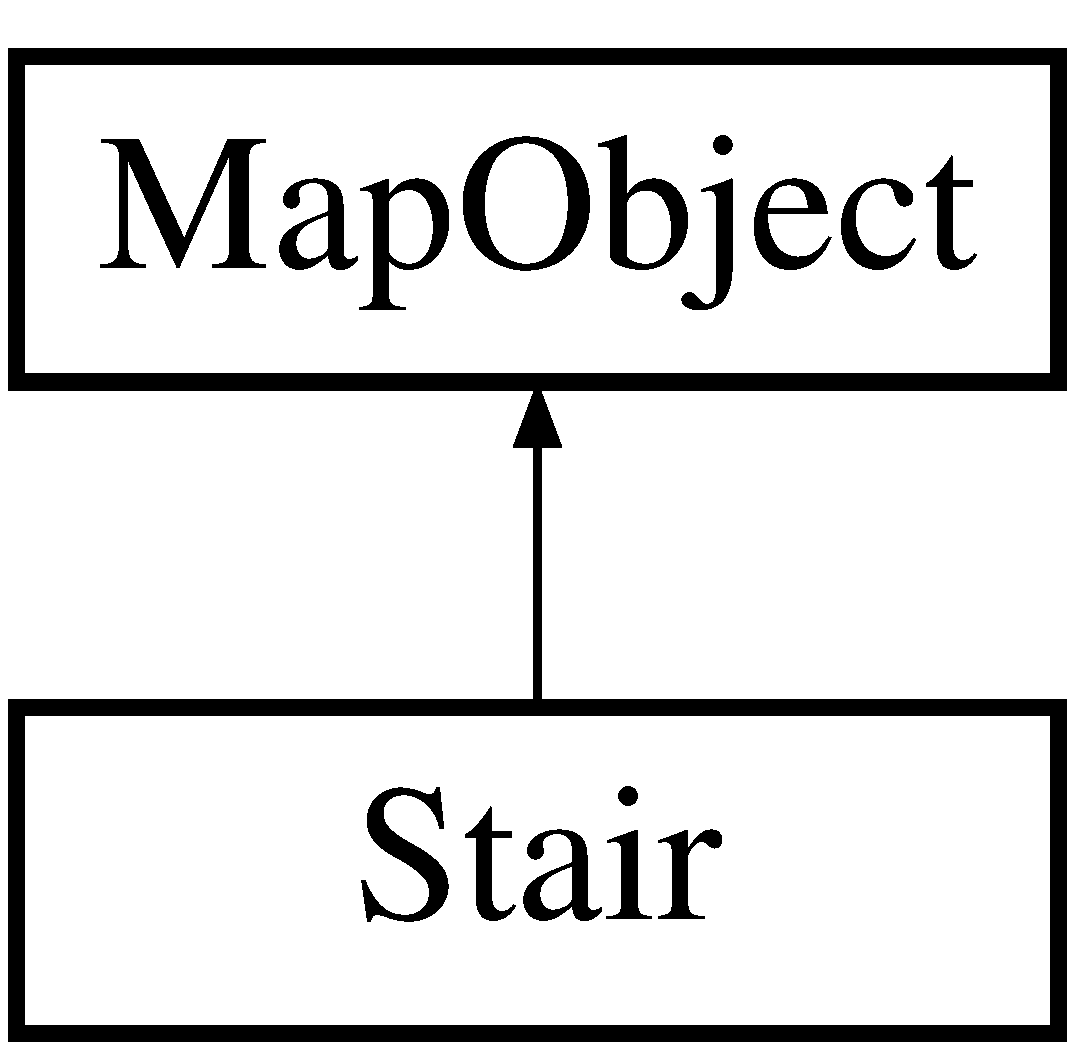
\includegraphics[height=2cm]{classStair}
\end{center}
\end{figure}
\subsection*{Public Member Functions}
\begin{CompactItemize}
\item 
{\bf Stair} (QString {\bf map\-Name}, int {\bf target\-X}, int {\bf target\-Y}, bool is\-Up, int {\bf tile})
\item 
virtual {\bf $\sim$Stair} ()
\item 
virtual QString {\bf get\-Class\-Name} () const 
\item 
QString {\bf get\-Map\-Name} () const 
\item 
int {\bf get\-Target\-X} () const 
\item 
int {\bf get\-Target\-Y} () const 
\item 
bool {\bf is\-Up} () const 
\end{CompactItemize}
\subsection*{Protected Attributes}
\begin{CompactItemize}
\item 
QString {\bf map\-Name}
\item 
int {\bf target\-X}
\item 
int {\bf target\-Y}
\item 
bool {\bf up}
\end{CompactItemize}


\subsection{Constructor \& Destructor Documentation}
\index{Stair@{Stair}!Stair@{Stair}}
\index{Stair@{Stair}!Stair@{Stair}}
\subsubsection{\setlength{\rightskip}{0pt plus 5cm}{\bf Stair} (QString {\em map\-Name}, int {\em target\-X}, int {\em target\-Y}, bool {\em is\-Up}, int {\em tile})}\label{classStair_a0}


\index{Stair@{Stair}!~Stair@{$\sim$Stair}}
\index{~Stair@{$\sim$Stair}!Stair@{Stair}}
\subsubsection{\setlength{\rightskip}{0pt plus 5cm}$\sim${\bf Stair} ()\hspace{0.3cm}{\tt  [virtual]}}\label{classStair_a1}




\subsection{Member Function Documentation}
\index{Stair@{Stair}!getClassName@{getClassName}}
\index{getClassName@{getClassName}!Stair@{Stair}}
\subsubsection{\setlength{\rightskip}{0pt plus 5cm}QString get\-Class\-Name () const\hspace{0.3cm}{\tt  [virtual]}}\label{classStair_a2}




Implements {\bf Map\-Object} {\rm (p.\,\pageref{classMapObject_a0})}.\index{Stair@{Stair}!getMapName@{getMapName}}
\index{getMapName@{getMapName}!Stair@{Stair}}
\subsubsection{\setlength{\rightskip}{0pt plus 5cm}QString get\-Map\-Name () const}\label{classStair_a3}


\index{Stair@{Stair}!getTargetX@{getTargetX}}
\index{getTargetX@{getTargetX}!Stair@{Stair}}
\subsubsection{\setlength{\rightskip}{0pt plus 5cm}int get\-Target\-X () const}\label{classStair_a4}


\index{Stair@{Stair}!getTargetY@{getTargetY}}
\index{getTargetY@{getTargetY}!Stair@{Stair}}
\subsubsection{\setlength{\rightskip}{0pt plus 5cm}int get\-Target\-Y () const}\label{classStair_a5}


\index{Stair@{Stair}!isUp@{isUp}}
\index{isUp@{isUp}!Stair@{Stair}}
\subsubsection{\setlength{\rightskip}{0pt plus 5cm}bool is\-Up () const}\label{classStair_a6}




\subsection{Member Data Documentation}
\index{Stair@{Stair}!mapName@{mapName}}
\index{mapName@{mapName}!Stair@{Stair}}
\subsubsection{\setlength{\rightskip}{0pt plus 5cm}QString {\bf map\-Name}\hspace{0.3cm}{\tt  [protected]}}\label{classStair_p0}


\index{Stair@{Stair}!targetX@{targetX}}
\index{targetX@{targetX}!Stair@{Stair}}
\subsubsection{\setlength{\rightskip}{0pt plus 5cm}int {\bf target\-X}\hspace{0.3cm}{\tt  [protected]}}\label{classStair_p1}


\index{Stair@{Stair}!targetY@{targetY}}
\index{targetY@{targetY}!Stair@{Stair}}
\subsubsection{\setlength{\rightskip}{0pt plus 5cm}int {\bf target\-Y}\hspace{0.3cm}{\tt  [protected]}}\label{classStair_p2}


\index{Stair@{Stair}!up@{up}}
\index{up@{up}!Stair@{Stair}}
\subsubsection{\setlength{\rightskip}{0pt plus 5cm}bool {\bf up}\hspace{0.3cm}{\tt  [protected]}}\label{classStair_p3}




The documentation for this class was generated from the following files:\begin{CompactItemize}
\item 
{\bf stair.hpp}\item 
{\bf stair.cpp}\end{CompactItemize}
